% APPLICATION
% - Usage Theory
%       - Instead of dropping packets, the network device with RED will send messages to an application announcing congestion
%       - These announcements allow the CPS to adjust its behavior to allow better operation during the network fault.
%       - Network layout and design
%       - What are the goals of the successful operation of the CPS algorithm
%       - Balance the amount of K that accumlates, while maximizing the amount of work done.
%       - Describe the type of traffic we are accounting for
% - What happens on the receipt of a Soft ECN Message & Motivate this approach
% - What happens on the receipt of a hard ECN message & Motivate this approach
% - Justify why these approaches are good for the CPS.
% - Make sure there's mathy stuff about why this is better.
% - Justification using the models developed in the last paper--
%   - The congestion would normally cause RED to drop packets at a certain rate, we're entering a contract with the router to change behavior rather than having an omission rate.
% - Tune RED parameters based on Journal paper?

\section{Application}

\subsection{Usage Theory}
When the RED algorithm identifies congestion it must notify senders of that congestion.
Since the ECN fields in IPv4 are not available to applications running on the system, the notifications are multicast onto the source interface.
Additionally, since this approach is non-standard and most UDP applications would not understand the notification, we have opted to create an application that runs on the network device.
This application is responsible for generating the multicast message.
It also keeps a register of hosts which are running applications which support reacting to the ECN notification.

There are several reasons for this approach.
First, related work has shown that an ECN strategy without some other queue management scheme is not sufficient to prevent congestion.
By allowing real-time applications that decrease the number of messages for congestion special priority in the RED algorithm, we allow those applications to continue operating during congestion.
Additionally, in later sections, we demonstrate that this strategy allows the best strategy for managing congestion.
To do this, we show that in similar scenarios the process that does not react to the congestion does not gain the benefit of the congestion management.

When the RED algorithm detects congestion, it sends a multicast beacon to a group of interfaces informing of the level of congestion.
For similarity with the RED algorithm and the NS3 implementation, this notification is classified as either ``soft'' or ``hard''.
A soft notification is an indication that the congestion in the network is approaching a level where message delays and packet loss are possible.
A hard notification indicates that the congestion has reached a level where congestion will cause message delays or packet loss.
The notifications are rate limited so they do not flood the network.

\subsection{Group Management}

The group management module's execution schedule is broken into several periods of message generation and response windows.
A typical schedule is shown in Figure X.
Because the schedule of the DGI triggers the execution of group management modules approximately simultaneously, the traffic generated by modules is bursty.
The number of messages sent is $O(n^2)$, in a brief window, which is dependent on how well the clocks are synchronized in the system.
The duration on the response window is dependent on the amount of time it takes for messages to propagate to the hardest-to-reach process that the DGI hopes to group with.
Additionally, to contend with congestion, an additional slack must be added to allow the RED algorithm to detect congestion before it reaches a critical level.
This is schedule is shown in Figure X.

Figure \ref{fig:queue-types} depicts typical queueing behavior for a network device serving DGI processes under different circumstances.
Because the traffic generated by DGI modules is very bursty, the queue experiences a phenoma where the bursty traffic mixed with a steady background traffic causes the queue to fill.
With no background traffic, the impulse queues a large number of messages, but those messages are distributed in a timely manner.
When the background traffic is introduced, the queue takes longer to empty.
At a critical threshold, the queue does not empty completely before the next burst is generated by the DGI.
In this scenario, shown in Figure \ref{fig:queue-types}.\ref{queue-congested}, the queue completely fills and no messages can be distributed.
The RED algorithm and ECN are used to delay or prevent the queue from reaching this critical threshold.

\begin{figure}
    \centering
    \begin{subfigure}[t]{0.3\textwidth}
        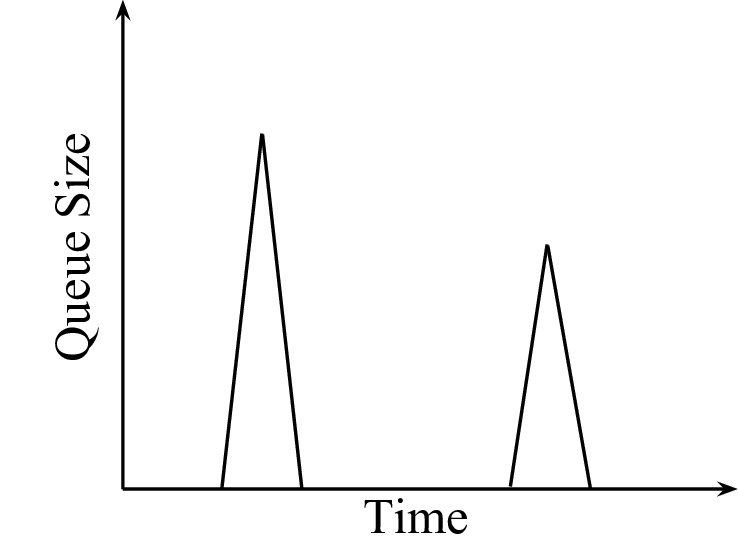
\includegraphics[width=\textwidth]{QueueNormal}
        \caption{When there is no other traffic on the network, the bursty traffic causes a large number of packets to queue quickly, but the queue empties a similiar rate.}
        \label{fig:queue-normal}
    \end{subfigure}
    ~ %add desired spacing between images, e. g. ~, \quad, \qquad, \hfill etc. 
      %(or a blank line to force the subfigure onto a new line)
    \begin{subfigure}[t]{0.3\textwidth}
        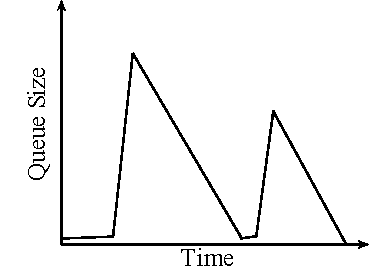
\includegraphics[width=\textwidth]{QueueTraffic}
        \caption{When there is other constant background draffic, the bursty traffic causes a large number of packets to be queued suddenly. More packets arrive continously, causing the queue to drain off more slowly.}
        \label{fig:queue-traffic}
    \end{subfigure}
    ~ %add desired spacing between images, e. g. ~, \quad, \qquad, \hfill etc. 
    %(or a blank line to force the subfigure onto a new line)
    \begin{subfigure}[t]{0.3\textwidth}
        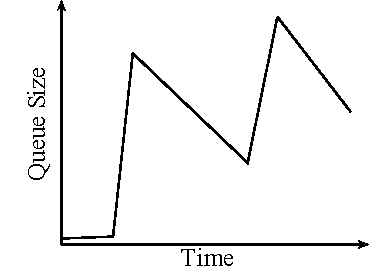
\includegraphics[width=\textwidth]{QueueCongested}
        \caption{When the background traffic reaches a certain threshold, the queue does not empty before the next burst occurs. When this happens, messages will not be delivered in time, and the queue will completely fill.}
        \label{fig:queue-congested}
    \end{subfigure}
    \caption{Example of network queueing during DGI operation. DGI modules are semi-synchronous, and create bursty traffic on the network.}\label{fig:queue-types}
\end{figure}

For this work, the algorithm from JOURNAL was used.
This algorithm has a higher message complexity than the Garcia-Molina algorithm which it is based on.
However, it does possess a desirable memoryless property that makes it easy to analyze.
This work uses an improved version of the algorithm which removes the restrictions in JOURNAL where only one process could become the leader.

\subsubsection{Soft ECN}

A soft ECN message indicates that the network has reached a level of congestion where the router suspects the process will not be able to meet its real time requirements.
The soft ECN message encourages the DGI processes to reduce the number of messages they send to reduce the amount of congestion they contribute to the network, and to allow for reliable distribution techinques to have additional time to deliver messages (since fewer messages are being sent).
In the case of potential congestion, the group managment module can reduce its traffic bursts by disabling elections during the congestion.
When the elections are disabled, messages for group management are only sent to members of the group.
Processes do not seek out better or other leaders to merge with.
As a consequence, the message complexity for processes responding to the congestion notification reduces from $O(n^2)$ to $O(n)$.

\subsubsection{Hard ECN}

In a hard ECN scenario, the router will have determined that congestion has reached a threshold where the real-time processes will soon not be able to meet their deadlines.
In this scenario, the real-time process will likely split its group.
In an uncontrolled situation, the split will be random.
It is therefore diserable when this level of traffic is reached to split the group.
Splitting the group reduces the number of messages sent across the router for processes with $O(N^2)$ message complexity.
For larger groups, splitting them provides a significant savings in the number of messages that must be queued by the router, especially since the traffic is very bursty.

\begin{figure}
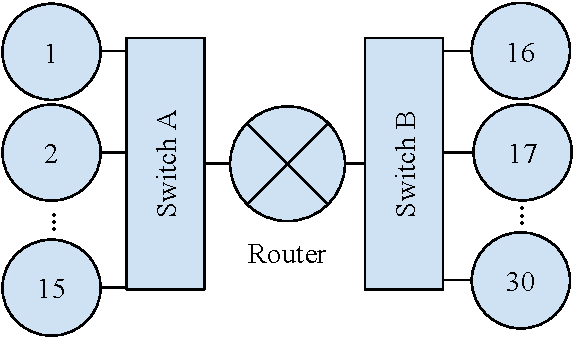
\includegraphics[width=\linewidth]{NetworkLayout}
\caption{Example of process organization used in this paper. Two groups of processes are contected by a router.} \label{fig:network-layout}
\end{figure}

Suppose a network like one depicted in Figure \ref{fig:network-layout}, where processes are divided by a router.
In Figure \ref{fig:network-layout}, there are $n$ processes on one side of the network and $m$ on the other.
In normal operation the omission-modelable algorithm has an $O(n^2)$ message complexity.
In Soft ECN matainence mode, the reduced number of messages reduces the complexity to $O(n)$ by disabling elections.

It is simple to observe that during the semi-synchronous execution of a $O(n)$ application, $c(m+n)$ messages are sent in each burst.
If the group is divided, an even mix of processes in the $n$ group and the $m$ group reduces the number of messages from $A->B$ and $B->A$ by at most $0.5$.
A worst case split does not reduce the number of messages travelling from $A->B$ or $B->A$
However, the benefit of group division is not mainly gained in the election algorithm, but rather the load balancing algorithm.
It will be shown in subsequent sections that there is a benefit to reduced groups for the load balancing algorithm due to its $O(n^2)$ complexity.

During elections (and with each group update) the leader distributes a fallback configuration that will coordinate the division of the groups during intense congestion.
When the ECN the notification is received the processes will halt all current group managment operations and enter a splitting mode where they switch to the fallback configuration.
The leader of the gorup distributes an Fallback notification to ensure that all processes in the group apply their new configuration. 
The complexity of distributing the notification is linear $O(n)$ and processes that already received the notification will have halted their communication.
This approach will ideally avoid the burst/drain phenoma from figure X.

The design of the fallback configuration can be created to optimize various factors.
These factors include cyber considerations, such as the likely network path the processes in the group will use to communicate.
By selecting the group around the network resources, the group can be selected to minimize the amount of traffic that crosses the congested links in the future.
Additionally, considerations from the physical network can be considered.
Fallback groups can be created to ensure that they can continue to facilitate the needs of the members.
This can take into the consideration the distribution of supply and demand processes in the current group.
By having a good mix of process types in the fallback group the potential for work can remain high.

From Equation X, it can be observed that the worst case reduction in link utilization for an $O(n^2)$ cut is UHHH.
This cut is affected by the

\subsection{Cyber-Physical System}

For a real-time cyber-physical system, message delays could mean that coordinated actions do not happen at the correct moments or not at all.
Since the two-generals problem prevents any process from being entirely certain that a coordinated action will happen in concert, problems arising from delay or omission of messages is of particular interest.
In particular, we are interested in the scenario from HARINI, where only half of a power migration is performed.
More other power managment algorithms could have similiar effects on the power system based on this idea of a process performing an action that is not compensated for by other processes.

\subsubsection{Soft ECN}

In a soft congestion notification mode, the process being informed of the congestion can reduce it's affect on the congestion by changing how often it generates bursty traffic.
Shown in Figure X, a processes running the load balancing algorithm make several traffic bursts when they exchange state information and prepare migrations.
As shown before, if the interval between these bursts is not sufficent for the queue to drain before the next burst occurs, then critical, overwhelming congestion occurs.
Since the schedule of the DGI is fixed at run-time processes cannot simply extend the duration of the load balancing execution phase.
However, on notification from the leader, the process can, instead, adjust the number of migrations to increase the sending gap.
This notification to reduce schedule originates from the coordinator as part of the message exchange neccessary for the process to remain in the group.
Every process in the group must receive this message to participate in load balancing, ensuring all processes remain on the same real-time schedule.
This reduced migration techinque and its effect on the schedule is shown in Figure X.
Using this approach, the amount of traffic generated is unchanged but the time period that a process waits for the messages to be distributed is increased.

\subsubsection{Hard ECN}

When the DGI process receives a hard congestion notification, the processes switch to a predetermined fallback configuration.
This configuration creates a cyber partition.
By partitioning the network, the number of messages sent by applications with $O(n^2)$ message complexity can be reduced significantly.
Each migration of load balancing algorithm begins with an $O(n^2)$ message burst and so benefits from the reduced group size created by the partition.

In the worst case scenario, some cut will have a single process opposite a large number of processes.
Suppose there is a network like the in Figure X with $n$ processes on one half and $m$ on the other.
Consider cut where one process is selected from side A and $m-1$ are selected from side B.
The cut will also create a second group of $n-1$ processes from side A and one process from side B.
The number of messages sent across the router for the undivided group is of the order $2mn$ as the $n$ processes on side A send a messsage to the $m$ on side B and vice-versa.
Let $i_{1}$ and $j_{1}$ be the number of processes from side A and side B (respectively) in the first group created by the partition.
Let $i_{2}$ and $j_{2}$ be the number of processes in the second group created by the partition under the same circumstances of $i_1$ and $j_1$.
The number of messages sent that pass through the router, is then 

\begin{equation}
2 i_{1} j_{1} + 2 i_{2} j_{2}
\end{equation}

The decrease in the number of message for this worst case partion is plotted in Figure X.
For an aribrary cut, the following can be observed.
Suppose $i_{1}$ and $j_{2}$ are the cardinaly of two arbitrarily chosen sets of processes from side A and side B respectively.
Following the same cut requirements as before:

\begin{equation}
i_2 = n - i_1
\end{equation}
\begin{equation}
j_2 = m - j_1
\end{equation}

The the number of messages that must pass through the router for this cut is:

\begin{equation}
2 i_{1} j_{1} + 2 (n-i_{1}) (m-j_{1})
\end{equation}
\begin{equation}
= 2 i_{1} j_{1} + 2 (nm - mi_{1} - nj_{1} + i_{1}j_{1})
\end{equation}
\begin{equation}
= 2 (2 i_{1} j_{1} + nm - mi_{1} - nj_{1})
\end{equation}

The value is minimized when $i_1$ and $j_1$ are $\frac{n}{2}$ and $\frac{m}{2}$:

\begin{equation}
2( 2 \frac{mn}{4} + mn - \frac{mn}{2} - \frac{mn}{2})
\end{equation}
\begin{equation}
= mn
\end{equation}

Which is a reduction of half as many messages.
For systems with a large number of participating processes this represents a significant reduction in the number of messages sent across the router.
As a consequence, this further extends the delivery window for processes sending messages.


\subsection{RED}
\subsubsection{Soft ECN}
\subsubsection{Hard ECN}
